\documentclass[a4paper,12pt]{article}   % papír A4, písmo 12 bodu
\usepackage[utf8x]{inputenc}             %kodovaní UTF-8
\usepackage{ucs}                        %kodovani unicode
\usepackage[czech]{babel}               %podpora cestiny
\usepackage[T1]{fontenc}                %pouzij variantu pisma T1 (hacky, carky)
\usepackage[left=2.5cm,right=1.5cm,top=2.5cm,bottom=2.5cm]{geometry} %okraje stranky
\usepackage{amsmath,amsfonts,amssymb}   %podpora matematiky
\usepackage{gensymb,marvosym}           %symboly celsius (\celsius) apod.
%\usepackage{mathptmx}                   %font Times New Roman s~podporou matematiky
\usepackage{times}                      %font Times New Roman (matematika pismem Computer Modern) 
\usepackage{parskip}                    %mezera mezi odstavci
%\usepackage[document]{ragged2e}         %text zarovany vlevo
\usepackage[none]{hyphenat} \sloppy     %slova nedelit a~nepretekat
\usepackage{titlesec}
\setcounter{secnumdepth}{4}
\clubpenalty 10000                      %kontrolovat sirotky
\widowpenalty 10000                     %kontrolovat vdovy
\usepackage{setspace} \onehalfspacing   %podpora pro zmenu radkovani + radkovani 1,5
\usepackage{enumerate}                  %podpora pro zmenu cislovani
\usepackage{fancyhdr}                   %vlastni zahlavi a~zapati
\usepackage{graphicx}                   %podpora grafiky
\graphicspath{{materialy/}}                   %vychozi adresar s~obrazky
\usepackage{caption}                    %popisky
\usepackage{subcaption}                 %podpopisky
\usepackage{siunitx}
\usepackage{MnSymbol,wasysym}
\usepackage[shortlabels]{enumitem}
\usepackage{amsmath}
\usepackage{lastpage}                   %zjištění poslední stránky \pageref{LastPage}
\usepackage{float}                      
\usepackage{url}
\usepackage[unicode]{hyperref}          %klikaci odkazy v~textu
\usepackage{mhchem}
\usepackage{multirow}

\usepackage{halloweenmath}


\titleclass{\subsubsubsection}{straight}[\subsection]
\newcounter{subsubsubsection}[subsubsection]
\renewcommand\thesubsubsubsection{\thesubsubsection.\arabic{subsubsubsection}}
\renewcommand\theparagraph{\thesubsubsubsection.\arabic{paragraph}} % optional, useful if paragraphs are to be numbered


%------------------------ čtvrtá a~pátá úroveň nadpisu ---------------------------

\titleformat{\subsubsubsection}
  {\normalfont\normalsize\bfseries}{\thesubsubsubsection}{1em}{}
\titlespacing*{\subsubsubsection}
{0pt}{3.25ex plus 1ex minus .2ex}{1.5ex plus .2ex}

\makeatletter

\renewcommand\paragraph{\@startsection{paragraph}{5}{\z@}%
  {3.25ex \@plus1ex \@minus.2ex}%
  {-1em}%
  {\normalfont\normalsize\bfseries}}
\renewcommand\subparagraph{\@startsection{subparagraph}{6}{\parindent}%
  {3.25ex \@plus1ex \@minus .2ex}%
  {-1em}%
  {\normalfont\normalsize\bfseries}}
\def\toclevel@subsubsubsection{4}
\def\toclevel@paragraph{5}
\def\toclevel@paragraph{6}
\def\l@subsubsubsection{\@dottedtocline{4}{7em}{4em}}
\def\l@paragraph{\@dottedtocline{5}{10em}{5em}}
\def\l@subparagraph{\@dottedtocline{6}{14em}{6em}}
\makeatother

\setcounter{secnumdepth}{4}
\setcounter{tocdepth}{4}


\setlist[enumerate]{itemsep=0mm}
%_____________________________|___________________________|_____________________________%
%                             |                           |                             %
%-----------------------------| ZDE VYPLNIT UDAJE O PRACI |-----------------------------%
%_____________________________|___________________________|_____________________________%
%                             

\newcommand{\nazev}{Měření odporů}                                                        %
\newcommand{\jmeno}{Jakub Dvořák}                                                     %
\newcommand{\datum}{20.11.2020}                                                              %
%---------------------------------------------------------------------------------------%


%-----------------------------| POUŽITÁ MAKRA |-----------------------------%

%\newcommand{\zkratka}{ve výsledku se mi napíše tenhle text}
%\newcommand{}{}
%\newcommand{}{}
%\newcommand{}{}
\newcommand{\tsub}[1]{$_\textrm{#1}$}
\newcommand{\texp}[1]{$^\textrm{#1}$}
\newcommand{\tohm}{$\Omega$}
\newcommand{\tmu}{$\mu$}
\newcommand{\var}[2]{$#1_\text{#2}$}
\renewcommand{\t}[1]{\text{#1}}
\newcommand{\sub}[1]{_{\text{#1}}}
\newcommand{\rxi}{R\sub{X\tsub{1}}}
\newcommand{\rxii}{R\sub{X\tsub{2}}}
\newcommand{\rx}{R\sub{X}}
\newcommand{\rn}{R\sub{N}}
\newcommand{\ui}{U\sub{1}}
\newcommand{\uii}{U\sub{2}}
\newcommand{\ii}{I\sub{1}}
\newcommand{\iii}{I\sub{2}}
\newcommand{\uijd}{U\sub{I\tsub{1,2}}}
\newcommand{\urx}{U\sub{R\tsub{X}}}
\newcommand{\urn}{U\sub{R\tsub{N}}}




%_______________________________________________________________________________________%
%_______________________________________________________________________________________%


%----------------------------------- KONEC PREAMBULE -----------------------------------%






%-------------------------------------- DOKUMENT --------------------------------------%
%______________________________________________________________________________________%
\begin{document} %%%%%%%%%%%%%%%%%%%%%%%%%%%%%%%%%%%%%%%%%%%%%%%%%%%%%%%%%%%%%%%%%%%%%%%

\setcounter{page}{0} %cislo strany
\pagestyle{empty} %stranku necislovat

%prostredi pro grafy a~schemata \begin{graf} \begin{schema}
\newfloat{schema}{htbp}{schema}\floatname{schema}{Schéma}
\newfloat{graf}{htbp}{graf}\floatname{graf}{Graf}

\begin{titlepage}
    \begin{center}
        \vspace*{1cm}
            
        \Huge
        \textbf{\nazev}
            
        \vspace{0.5cm}
        \LARGE
            
        \vspace{1.5cm}
            
        \textbf{\jmeno}
            
        \vfill
            
        \vspace{0.8cm}
            
        \Large
            
        \datum\\
        \vspace*{.5cm}
        
\includegraphics[width=.4\textwidth]{logo-cvut-fee.png}\\
    \end{center}
\end{titlepage}

% --- definice zapati a~cislovani ---
\newpage 
\pagestyle{fancy}                                       %vlastni zahlavi/zapati
\renewcommand{\headrulewidth}{0pt}                      %bez linky v~zahlavi
\renewcommand{\footrulewidth}{.5pt}                    %linka v~zapati - optional
\lhead{}       \chead{} \rhead{\nazev}                        %pole zahlavi (prazdna)
\lfoot{\jmeno} \cfoot{} \rfoot{\thepage}   %pole zapati


%------------------------------------ VLASTNÍ TEXT ------------------------------------%



\section{Úkol měření}
\label{chap:ukol}
\begin{enumerate}
    \item 
    \begin{enumerate}[label=\alph*)]
        \item Měření malých odporů Ohmovou metodou. Sestavte měřicí obvod dle obr. 1. Vhodnou metodikou měření vylučte vliv termoelektrických napětí. Z naměřených hodnot napětí a~proudu vypočtěte velikost neznámého odporu \var{R}{X} a stanovte rozšířenou nejistotu měření (pro \var{k}{R}~=~2).
        \item Měření malých odporů sériovou srovnávací metodou. Zapojte měřicí obvod dle obr. 2. Změřte napětí na etalonu \var{R}{N} a napětí na měřeném odporu \var{R}{X}. Vhodnou metodikou měření vylučte vliv termoelektrických napětí. Vypočtěte velikost neznámého odporu \var{R}{X} a odvoďte vztah pro nejistotu měření.
        \item Měření středních odporů převodníkem R \var{\rightarrow}{} U. Sestavte převodník odpor-napětí s OZ (\var{U}{R}~=~10 V, \var{R}{N1}~=~10 k\tohm ) dle obr. 3. Odvoďte přenos převodníku a ověřte jeho funkci. Jako odpor \var{R}{X} použijte odporovou dekádu. Zdůvodněte, do jaké hodnoty odporu může uvedený převodník měřit.
    \end{enumerate}
\end{enumerate}


\section{Schéma zapojení}
\label{chap:schema_zapojeni}
\begin{figure}[h!]
  \centering
  \begin{minipage}{.4\textwidth}
    \centering
    \captionsetup{width=0.8\textwidth}
    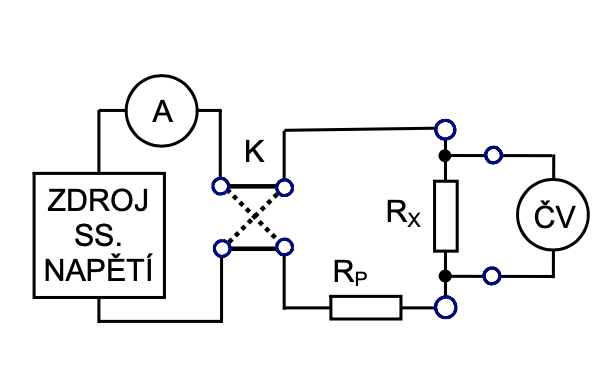
\includegraphics[width=\textwidth]{ohm.png}
    \caption{Měření malého odporu Ohmovou metodou}
    \label{fig:ohm}
  \end{minipage}
  \begin{minipage}{.4\textwidth}
    \centering
    \captionsetup{width=0.8\textwidth}
    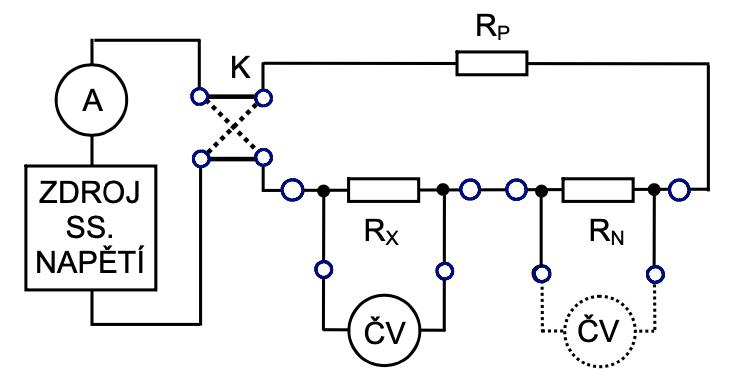
\includegraphics[width=\textwidth]{ser.png}
    \caption{Měření malého odporu sériovou metodou}
    \label{fig:ser}
  \end{minipage}
\end{figure}

\begin{figure}
  \centering
  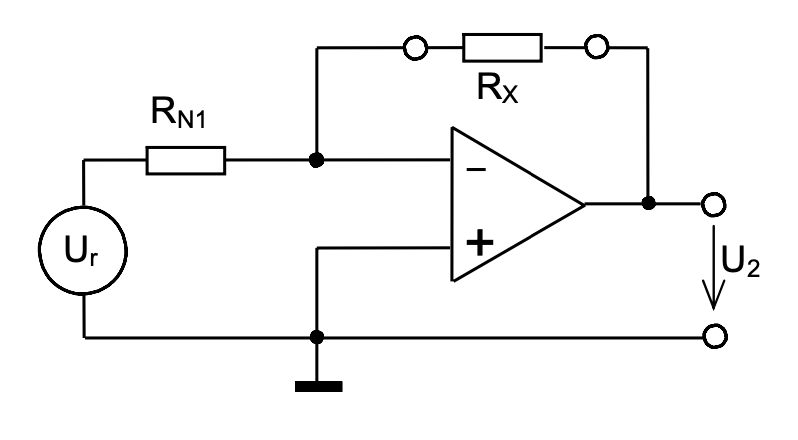
\includegraphics[width=.4\textwidth]{ru.png}
  \caption{Převodník R $\rightarrow$ U}
\end{figure}


\section{Seznam použitých přístrojů}
\label{chap:seznam_pristroju}
\begin{enumerate}
  \item Laboratorní zdroj Agilent Proud < 0,2 \% z hodnoty + 10 mA
  \item Digitální voltmetr HP 34401A \var{\pm}{} 0,0050 \% údaje \var{\pm}{} 0,0035 \% rozsahu
\end{enumerate}




\section{Teoretický úvod}
\label{chap:teoreticky_uvod}
Při měření malých odporů se uplatňuje i přechodový odpor mezi zdrojem proudu a měřeným odporem. Pro eliminaci tohoto jevu se používá tzv. \textit{čtyřsvorková} metoda. Pro vyloučení jevu termoelektrických jevů, jejich velikost je závislá na směru proudu, měříme oba směry. Následně výsledný odpor vypočítáme jako aritmetický průměr naměřených hodnot. $\rx=\frac{\left(\rxi+\rxii\right)}{2}$. Pro měření ohmovou metodou použijeme vzorec $\rx=\frac{U}{I}$ a pro měření srovnávací metodou využijeme vzorec $\rx = \frac{\urx}{\urn}\cdot\rn$.


\section{Naměřené hodnoty}
\label{chap:namerene_hodnoty}
Naměřené hodnoty jsou níže v tabulkách:


\begin{table}[h!]
  \centering
  \begin{subtable}[t]{.4\textwidth}
    \centering
    \begin{tabular}{|r|c|c|}
      \hline
      \multicolumn{3}{|c|}{Sériová srovnávací metoda}\\\hline\hline
      $U\sub{R\tsub{N}}$ (V)	&	$U\sub{R\tsub{X}}$ (V)	&	$R_\text{X}$ (m\tohm)	\\\hline
      0,876   &	10,082	  &	11,509	    \\\hline
      0,896   &	10,251	  &	11,441	    \\\hline\hline
      \multicolumn{3}{|c|}{$\rx=11,475$ m\tohm}\\\hline
    \end{tabular}
    \caption{Odpor vypočtený srovnávací metodou}
    \label{tab:srov}
  \end{subtable}
  \begin{subtable}[t]{.4\textwidth}
    \centering
    \begin{tabular}{|r|c|c|}
      \hline
      \multicolumn{3}{|c|}{Ohmova metoda}\\\hline\hline
      $I$ (A)	&	$U$ (V)	&	$R$ (m\tohm)	\\\hline
      1	      &	11,3	  &	11,3	    \\\hline
      -1	    &	11,7	  &	11,7	    \\\hline\hline
      \multicolumn{3}{|c|}{$\rx=11,5$ m\tohm}\\\hline
    \end{tabular}
  \caption{Odpor vypočtený Ohmovou metodou}
  \label{tab:ohm}
  \end{subtable}
  \begin{subtable}[]{\textwidth}
    \begin{tabular}{c}
      \\
    \end{tabular}
  \end{subtable}
  \begin{subtable}[]{.4\textwidth}
    \centering
    \begin{tabular}{|r|c|c|}
      \hline
      \multicolumn{3}{|c|}{Měření převodníkem U \var{\rightarrow}{} I}\\\hline\hline
      $U\sub{out}$ (V)	&	$U\sub{in}$ (V)	&	$R_\text{X}$ (k\tohm)	\\\hline
      5   &	-5,99	  &	11,980	    \\\hline\hline
      \multicolumn{3}{|c|}{$\rx=11,980$ k\tohm}\\\hline
    \end{tabular}
    \caption{Odpor změřený převodníkem U \var{\rightarrow}{} I}
    \label{tab:prevod}
  \end{subtable}
\end{table}

\section{Zpracování naměřených hodnot}
\label{chap:zpracovani_hodnot}
\begin{equation}
  u_\text{U$_\text{1,2}$}=\frac{\frac{\delta_1}{100}\cdot X+\frac{\delta_2}{100}\cdot M}{\sqrt{3}} = \frac{\frac{0,005}{100}\cdot 10,082+\frac{0,0035}{100}\cdot 100}{\sqrt{3}} = 2,3~\mu\text{V}
\end{equation}
\begin{equation}
  u_\text{I$_\text{1,2}$}=\frac{\frac{\delta_1}{100}\cdot X+\frac{\delta_2}{100}\cdot M}{\sqrt{3}} = \frac{\frac{0,2}{100}\cdot 1 + 10\cdot 10^{-3}}{\sqrt{3}} = 6,9~\text{mA}
\end{equation}
\begin{equation}
  u_{\text{R}_{\text{X}_\text{1}}}~=~\sqrt{\left(\frac{\partial R_\t{x}}{\partial I}\cdot u_{\t{I}_{\t{1,2}}}\right)^2 + \left(\frac{\partial R_\t{x}}{\partial U}\cdot u_{\t{U}_{\t{1,2}}}\right)^2} = \sqrt{\left(-\frac{U}{I} \cdot u_{\t{I}_{\t{1,2}}} \right)^2 + \left(\frac{1}{I} \cdot u_{\t{U}_{\t{1,2}}} \right)^2} = 7,8\cdot 10^{-5}~\Omega
\end{equation}
Můžeme předpokládat, že nejistoty měření budou velice podobné pro oba směry proudu. Výsledná nejistota tedy vyjde
\begin{equation}
  u_{\t{R}_\t{X}}=\frac{u_{\text{R}_{\text{X}_\text{1}}}}{\sqrt{2}}
\end{equation}
Výsledná nejistota s koeficientem rozšíření poté bude
\begin{equation}
  U_{\t{R}_\t{X}}=k_r\cdot \frac{7,8\cdot 10^{-5}}{\sqrt{2}} = 1,1\cdot 10^{-4}~\Omega
\end{equation}



\section{Závěrečné vyhodnocení}
\label{chap:zaver}



%--- LITERATURA a~ZDROJE (povinne) ---
\clearpage
\renewcommand{\refname}{Seznam použité literatury a~zdrojů informací} 
%\section*{Seznam použité literatury a~zdrojů informací}
\phantomsection %pridej odkaz do PDF zalozek
\addcontentsline{toc}{section}{Seznam použité literatury a~zdrojů informací}

\begin{thebibliography}{99}

%----------------------------------------------------
\subsection*{Seznam použitých internetových zdrojů}
    \bibitem{navod} Návod k~laboratorní úloze
    
\end{thebibliography}

\end{document}